% !TEX root = ../main.tex
%
\chapter{Technical Implementation}
\label{sec:system}

\section{System Architecture}
\label{sec:system:architecture}

% Technology Stack Rational
% Architecture Diagram & data flow

The architecture followed a standard client server pattern, with the server functioning as a wrapper for the nerfstudio CLI, and the client as a web application.
The server was built using tRPC, a framework for building type-safe APIs in TypeScript.
It was responsible for handling incoming requests from the client, and translating them into commands that the nerfstudio CLI could understand.
Requests from the client were sent to the server using HTTP requests, and in case of an asynchronous operation, the server would update the client on using websockets.

\begin{figure}[htb]
	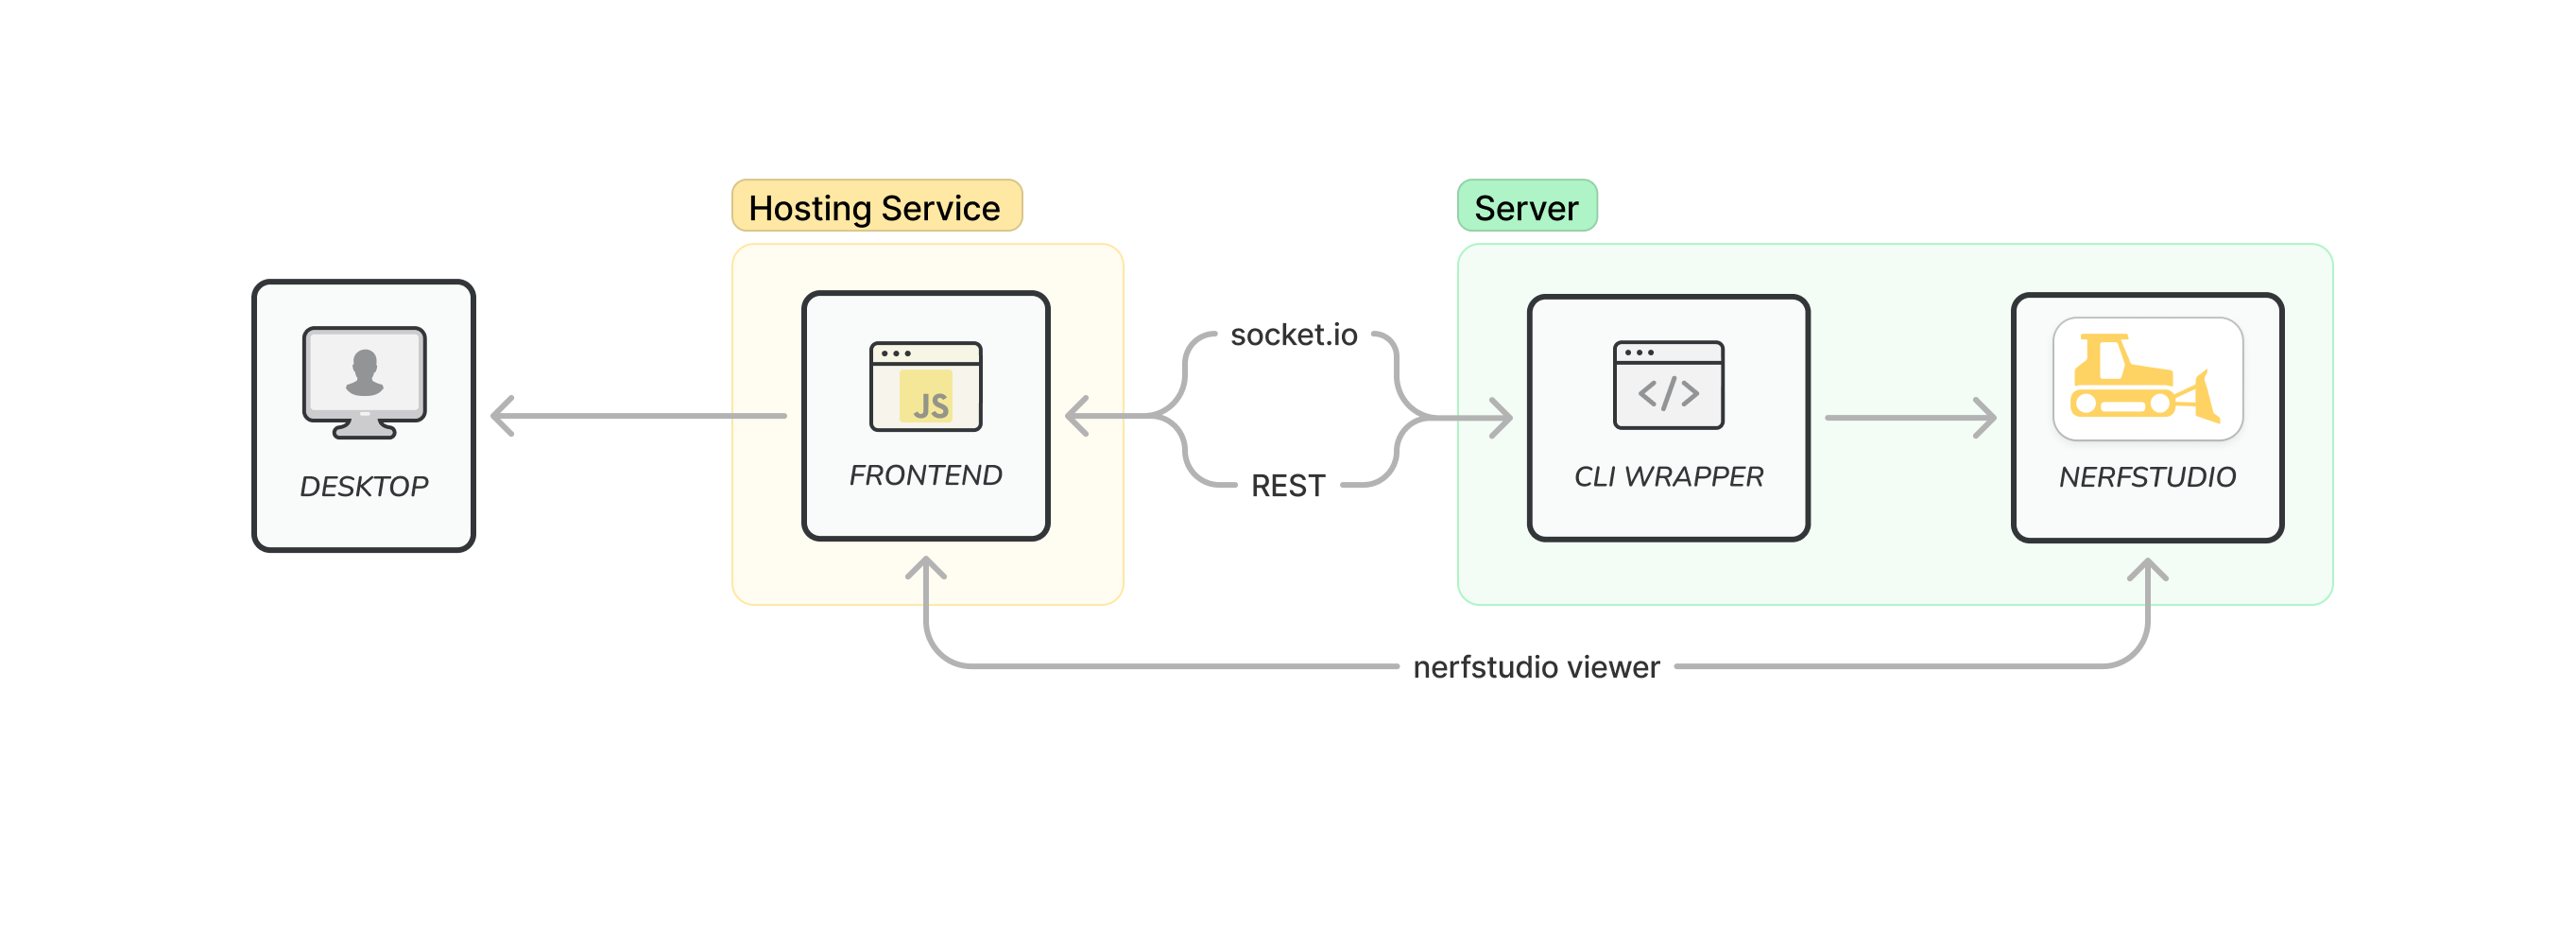
\includegraphics[width=\textwidth]{figures/architecture-1.png}
	\caption{System Architecture}
	\label{fig:system:example2}
\end{figure}

For the prototype, all the components were composed into a single docker container and deployed as a single unit.
This leveraged the pre-configured container provided by nerfstudio, and allowed for a quick and easy deployment of the prototype.

\section{Frontend Development} 
\label{sec:system:frontend}

% Setup, configuration, and component architecture
% UI/UX design principles

The frontend was built with React, as it is a popular and well supported framework for building web applications.
Vite was used as a build tool, as it provides a fast and efficient development experience.
To accelerate the styling process, Tailwind CSS was used, it is a utility-first CSS framework that provides a set of pre-defined classes that can be used to style components.
In additional the daisyUI component library provided a set of pre-styled components that could be used to quickly build the UI.

\subsubsection{Extensibility}

Extensibility was a key considerations during the development of the frontend, as the underlying nerfstudio CLI is in itself extendable.
All parameters for processing and training a NeRF model are configurable using JSON or strongly typed TypeScript objects.

\begin{lstlisting}[caption=Parameter Option configuration]
const stepsPerSave: NumberInput = {
	name: "stepsPerSave",
	label: "Steps Per Save",
	tooltip: "Number of steps between each save of the model.",
	inputType: "number",
	defaultValue: 1000,
};
\end{lstlisting}

Currently the supported input types are: number, select and boolean, but it is easy to add new types by extending the configuration object. 
It is also possible to define dependent parameters, that are only shown when a certain condition is met.
Images to illustrate the effect of a parameter can be added as well, to provide additional context to the user.

Filters and presets are also configurable using arrays of the names of the parameters that should be included in the filter or preset.
The full configuration can be found in the \texttt{frontend/src/config} folder in the codebase.

\subsubsection{Nerfstudio Viewer Integration}

The nerfstudio viewer is built using Viser, a library for building 3D visualizations using python.
This posed some limitations in integrating it into the frontend, as it is not easily possible to directly embed a python application into a web application.
To work around this, the viewer was hosted by nerfstudio as usual and embedded into the frontend using an iframe.

Some modifications could be made to the viewer to make it more suitable for embedding.
This included some simple styling changes to make the viewer fit better into the frontend.
The viewer contained several interactions where it was necessary for the user to copy console commands, to be used in the CLI.
These interactions were replaced with buttons that send a request to the server to execute the command instead.

These modifications were done at build-time of the container by applying a patch to the nerfstudio source code of the base image.


\section{Backend Development}
\label{sec:system:backend}

% Advantages of tRPC, configuration, and API design

The backend was built using tRPC, a framework for building type-safe APIs in TypeScript.
This type-safety was useful in building the API, as nerfstudio endpoints require a specific set of parameters of various types, that could be easily defined using TypeScript and reused in the frontend.

With tRPC, 

\section{Challenges and Solutions}
\label{sec:system:challenges}


\section{Lessons Learned}
\label{sec:system:lessons}

\section{Future Directions}
\label{sec:system:future}
